\subsection{Procesory, multiprocesory}

\begin{definiceN}{Procesor} 
Procesor (CPU – central processing unit) je ústřední výkonnou jednotkou počítače, která čte z paměti instrukce a na jejich základě vykonává program.

Základnými súčasťami procesora sú:
\begin{pitemize}
	\item řadič nebo řídicí jednotka, která řídí tok programu, tj. načítání instrukcí, jejich dekódování, načítání operandů instrukcí z operační paměti a ukládání výsledků zpracování instrukcí
	\item sada registrů k uchování operandů a mezivýsledků.
	\item jedna nebo více aritmeticko-logických jednotek (ALU), které provádí s daty aritmetické a logické operace.
	\item některé procesory obsahují jednu nebo několik jednotek plovoucí čárky (FPU), které provádí operace v plovoucí řádové čárce.
\end{pitemize}
\end{definiceN}

\begin{poznamka}
Súčasné procesory navyše často obsahujú ďalšie rozsiahle funkčné bloky (cache, rôzne periférie)~-- ktoré z \uv{ortodoxného hladiska} nie sú priamo súčasťou \emph{jadra procesoru}. Niektoré procesory môžu obsahovať viac jadier (+logiku slúžiacu k ich vzájomnému prepojeniu). Ďalším trendom je SoC (System on Chip), kde sa na čipe procesora nachádzajú aj ďalšie subsystémy napr. na spracovanie zvuku, grafiky alebo pripojenie externých periférií (takéto riešenia sa využívajú väčšinou v PDA, domácej elektronike, mobiloch atď.).
\end{poznamka}

\begin{obecne}{Dělení podle instruční sady}
Podľa inštrukčnej sady je možné procesory rozdeliť na:
\begin{pitemize}
	\item \textbf{CISC} (Complex Instruction Set Computer): poskytuje rozsiahlu inštrukčnú sadu spolu s rôznymi variantami inštrukcií. Jedna inštrukcia napr. môže vykonať veľa low-level operácií (načítanie z pamäti, vykonať aritmetickú operáciu a výsledok uložiť). Takéto inštrukcie zjednodušovali zápis programov (inštrukcie boli bližšie vyšším programovacím jazykom) a zmenšovali veľkosť programu a počet prístupov do pamäti~-- čo bolo v 60tych rokoch dôležité. Avšak nie vždy je vykonanie jednej zložitej operácie rýchlejšie ako vykonanie viac menej zložitých miesto toho (napr. kvôli zložitému dekódovaniu a použitiu mikrokódu na volanie jednoduchých \uv{podinštrukcií}). Príkladmi CISC architektúr procesorov sú System/360, Motorola 68000 a Intel x86. V súčasnosti napr. x86 rozkladá zložité inštrukcie na \uv{micro-operations} ktoré môžu byť pipeline-ou spracované paralelne a vyšší výkon je tak dosahovaný na väčšom rozsahu inštrukcií. Vďaka tomu sú súčasné x86 procesory minimálne rovnako výkonné ako ozajstné RISC architektúry.
	\item \textbf{RISC} (Reduced Instruction Set Computer): design CPU ktorý uprednosňuje jednoduchšiu inštrukčnú sadu a menšiu zložitosť adresovacích modelov~-- vďaka čomu je možné dosiahnuť lacnejšiu implementáciu, väčšiu úroveň paralelizmu a účinnejšie kompilátory. Dôvodom vzniku bolo aj nevyužívanie celej CISC inštrukčnej sady a upredňostňovania len obmedzenej podmnožiny (designéri procesorov potom optimalizovali len tieto podmnožiny a tak sa zvyšné inštrukcie používali ešte menej...). Kvôli väčšiemu počtu inštrukcií však musia RISC procesory častejšie pristupovať k pamäti... Príkladmi RISC procesorov sú napr. SPARC a ARM. V architekturách typu \textbf{Post-RISC} jde o spojení RISCových vlastností s technikami zvýšení výkonu, jako je out-of-order vykonávání a paralelismus.
    \item \textbf{VLIW}: Very Long Instruction Word or VLIW refers to a CPU architecture designed to take advantage of instruction level parallelism (ILP). A processor that executes every instruction one after the other (i.e. a non-pipelined scalar architecture) may use processor resources inefficiently, potentially leading to poor performance. The performance can be improved by executing different sub-steps of sequential instructions simultaneously (this is pipelining), or even executing multiple instructions entirely simultaneously as in superscalar architectures. The VLIW approach, on the other hand, executes operation in parallel based on a fixed schedule determined when programs are compiled. Since determining the order of execution of operations (including which operations can execute simultaneously) is handled by the compiler, the processor does not need the scheduling hardware that the three techniques described above require. As a result, VLIW CPUs offer significant computational power with less hardware complexity (but greater compiler complexity) than is associated with most superscalar CPUs.
    \item \textbf{EPIC}: (Někdy označován za poddruh VLIW) Explicitly Parallel Instruction Computing (EPIC) is a computing paradigm that began to be researched in the 1990s. This paradigm is also called Independence architectures. It was used by Intel and HP in the development of Intel’s IA-64 architecture, and has been implemented in Intel’s Itanium and Itanium 2 line of server processors. The goal of EPIC was to increase the ability of microprocessors to execute software instructions in parallel, by using the compiler, rather than complex on-die circuitry, to identify and leverage opportunities for parallel execution. This would allow performance to be scaled more rapidly in future processor designs, without resorting to ever-higher clock frequencies, which have since become problematic due to associated power and cooling issues.
\end{pitemize}
\medskip
TODO: asi opravit, možná zpřesnit VLIW a EPIC a určitě přeložit

\medskip
Řekneme, že procesor má \emph{ortogonální instrukční sadu}, pokud žádná instrukce nepředpokládá implicitně použití některých registrů. To umožňuje jednodušší práci algoritmům přidělování registrů v překladačích. Příkladem neortogonální instrukční sady je i x86.
\end{obecne}

\begin{obecne}{Další dělení}
Ďalej je možné procesory rozdeliť podľa dĺžky operandov v bitoch (8, 16, 32, 64...), ktorý je procesor schopný spracovať v jednom kroku. V embedded zariadeniach sa najčastejšie používajú 4- a 8-bitové procesory. V PDA, mobiloch a videohrách 8 resp. 16 bitové. 32 a viac bitov využíajú napr. osobné počítače a laserové tlačiarne.

Dôležitou vlastnosťou je aj taktovacia frekvencia jadra, MIPS (millions of instructions per second) a jeho rýchlosť. V súčasnosti je ťažké dávať do súvislosti výkon procesorov s ich frekvenciou (resp. MIPS)~-- kým Pentium zvládne na výpočet vo floatoch, jednoduchý 8-bitový PIC na to potrebuje oveľa viac taktov. Ďalším \uv{problémom} je superskalarita procesorov, ktorá im umožňuje vykonať viacero nezávislých inštrukcií počas jedného taktu.
\end{obecne}

\begin{obecne}{Techniky pro zvýšení výkonu}
Zvyšovať výkon (procesorov) je možné viacerými spôsobmi. Najjednoduchším (a najpomalším) typom je Subskalárny CPU (načíta a spracúva len jednu inštrukciu naraz~-- preto musí celý procesor čakať kým vykonávanie inštrukcie skončí; je tak zdržovaný dlhšie trvajúcimi inštrukciami). 

\begin{center}
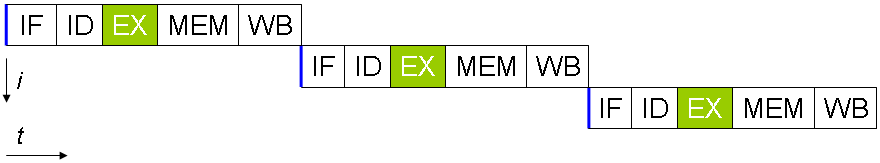
\includegraphics[width=8cm]{informatika/operacne_systemy_a_hw/obrazky/Nopipeline.png}
\end{center}

Pokusy o dosiahnutie skalárneho a lepšieho výkonu vyústili do designov ktoré sa správajú menej lineárne a viac paralelne. Čo sa týka paralelizmu v procesoroch, používajú sa dva druhy pojmov na ich klasifikáciu~-- \emph{Instruction level parallelism} (zvyšovanie rýchlosti vykonávania inštrukcií v procesore a teda zväčšovanie využitia prostriedkov na čipe) a \emph{Thread level parallelism} (zväčšovanie počtu vlákien, ktoré dokáže CPU vykonávať naraz).
\begin{pitemize}
  \item \textbf{pipeline}: 
  Zlepšenie je možné dosiahnúť pomocou \uv{instruction pipelining}-u, ktoré je použíté vo väčšine moderných procesorov. Umožňuje vykonanie viac ako jednej inštrukcie v jednom kroku vďaka rozloženiu spracovávania inštrukcie na viac menších krokov: 
  \begin{center}
  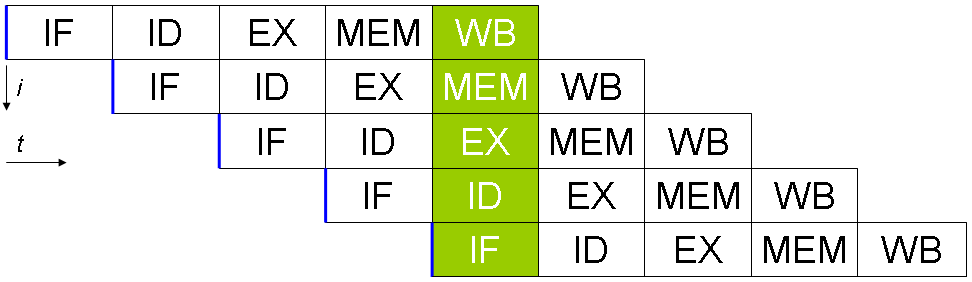
\includegraphics[width=8cm]{informatika/operacne_systemy_a_hw/obrazky/Fivestagespipeline.png}
  \end{center}

  \item \textbf{superskalarita}: Dialša možnosť je použitie superscalar designu, ktorý obsahuje dlhú inštrukčnú pipeline a viacero identických execution jednotiek.  
  \begin{center}
  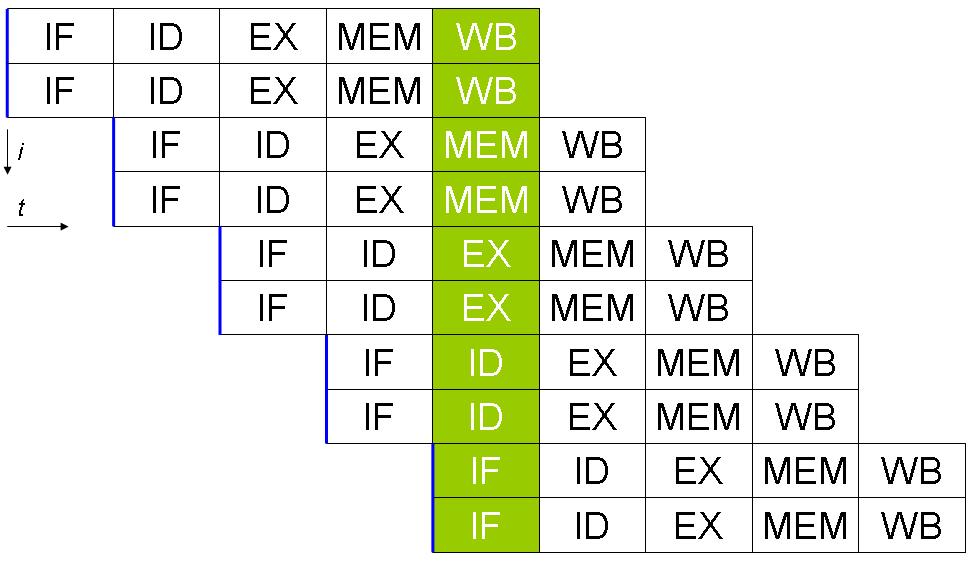
\includegraphics[width=8cm]{informatika/operacne_systemy_a_hw/obrazky/Superscalarpipeline.png}
  \end{center}	

  \item \textbf{Out of order execution}
  \begin{penumerate}
	  \item Načtení instrukce, případně její rozdrobení na mikroinstrukce
	  \item Zařazení do vyčkávací stanice (instruction pool)
	  \item Instrukce čeká na všechny svoje operandy
	  \item Instrukce se vykoná ve své výkonné jednotce (je vybírána z instruction poolu nezávisle na ostatních)
	  \item Výsledky se uchovají ve frontě (reorder buffer)
	  \item Až se všechny starší instrukce zapíší do registrů, zapíše se výsledek této instrukce (opětovné řazení)
  \end{penumerate}

  \item \textbf{Predikce skoků}~-- hluboké pipeliny mají problém, pokud podmíněný skok není proveden; dynamická predicke skoků (historie CPU~-- vzory nějaké hloubky) vs. statická (bez nápovědy~-- skok vpřed se neprovede, skok vzad se provede; s nápovědou~-- překladač odhaduje pravděpodobnost skoku)

  \item \textbf{Spekulativní vykonávaní}~-- vykonávání kódu, který nemusí být zapotřebí; významná disproporce mezi rychlostí CPU a paměti; typické využití je značné předsunutí čtecích operací; CPU provádí i odsouvání zápisových operací


  \item \textbf{Data parallelism}: SIMD inštrukcie (napr. multimediálne inštrukcie), vektorové procesory...
\end{pitemize}
\end{obecne}

\subsubsection*{Multiprocesory}

TODO: jde o copy \& paste z Wiki ... předělat česky/slovensky
\medskip

\begin{definiceN}{Multiprocesor}
  O \emph{multiprocesoru} mluvíme, pokud je použito dvou nebo více procesorů
  (CPU) v rámci jednoho počítačového systému. Termín je také používán mluvíme-li
  o schopnosti systému využívat více procesorů a/nebo schopnosti rozdělovat
  úlohy mezi jednotlivými procesory.
\end{definiceN}

\begin{obecne}{Vztah k datům a instrukcím}
In multiprocessing, the processors can be used to execute a single sequence of instructions in multiple contexts (single-instruction, multiple-data or SIMD, often used in vector processing), multiple sequences of instructions in a single context (multiple-instruction, single-data or MISD, used for redundancy in fail-safe systems and sometimes applied to describe pipelined processors or hyperthreading), or multiple sequences of instructions in multiple contexts (multiple-instruction, multiple-data or MIMD).
\end{obecne}

\begin{obecne}{Symetrie}
In a multiprocessing system, all CPUs may be equal, or some may be reserved for special purposes. A combination of hardware and operating-system software design considerations determine the symmetry (or lack thereof) in a given system. For example, hardware or software considerations may require that only one CPU respond to all hardware interrupts, whereas all other work in the system may be distributed equally among CPUs; or execution of kernel-mode code may be restricted to only one processor (either a specific processor, or only one processor at a time), whereas user-mode code may be executed in any combination of processors. Multiprocessing systems are often easier to design if such restrictions are imposed, but they tend to be less efficient than systems in which all CPUs are utilized equally.

Systems that treat all CPUs equally are called symmetric multiprocessing (SMP) systems. In systems where all CPUs are not equal, system resources may be divided in a number of ways, including asymmetric multiprocessing (ASMP), non-uniform memory access (NUMA) multiprocessing, and clustered multiprocessing (qq.v.).
\end{obecne}

\begin{obecne}{Těsnost spojení multiprocesorů}
\begin{pitemize}
    \item \textbf{Tightly-coupled} multiprocessor systems contain multiple CPUs that are connected at the bus level. These CPUs may have access to a central shared memory (SMP or UMA), or may participate in a memory hierarchy with both local and shared memory (NUMA). The IBM p690 Regatta is an example of a high end SMP system. Intel Xeon processors dominated the multiprocessor market for business PCs and were the only x86 option till the release of AMD's Opteron range of processors in 2004. Both ranges of processors had their own onboard cache but provided access to shared memory; the Xeon processors via a common pipe and the Opteron processors via independent pathways to the system RAM.

    \item \textbf{Chip multiprocessors}, also known as multi-core computing, involves more than one processor placed on a single chip and can be thought of the most extreme form of tightly-coupled multiprocessing. Mainframe systems with multiple processors are often tightly-coupled.

    \item \textbf{Loosely-coupled multiprocessor} systems (often referred to as clusters) are based on multiple standalone single or dual processor commodity computers interconnected via a high speed communication system (Gigabit Ethernet is common). A Linux Beowulf cluster is an example of a loosely-coupled system.
\end{pitemize}
Tightly-coupled systems perform better and are physically smaller than loosely-coupled systems, but have historically required greater initial investments and may depreciate rapidly; nodes in a loosely-coupled system are usually inexpensive commodity computers and can be recycled as independent machines upon retirement from the cluster.

\textbf{SMP} (Symmetric Multiprocessing): viac procesorov so zdieľanou operačnou pamäťou (nutné mechanizmy na zabránenie nesprávnych náhľadov na pamäť a migráciu procesov medzi procesormi). SMP systems allow any processor to work on any task no matter where the data for that task are located in memory; with proper operating system support, SMP systems can easily move tasks between processors to balance the workload efficiently.
\end{obecne}
